% Scoping Review Outline — Gut Microbiome and Time-to-GVHD in Adult Allo-SCT
% This is a working outline with figure placeholders and bullet-point content guides.
% Compile with: pdflatex -> biber -> pdflatex -> pdflatex
%%%%%%%%%%%%%%%%%%%%%%%%%%%%%%%%%%%%%%%%%%%%%%%%%%%%%%%%%%%%%%%%%%%

\documentclass[11pt,a4paper]{article}
\usepackage[margin=2.5cm]{geometry}
\usepackage[onehalfspacing]{setspace}
\usepackage{graphicx}
\usepackage[breaklinks=true,colorlinks=true,linkcolor=blue,urlcolor=blue,citecolor=blue]{hyperref}
\usepackage{amsmath,amssymb}
\usepackage[T1]{fontenc}
\usepackage{booktabs}
\usepackage{longtable}
\usepackage{array}
\usepackage{xcolor}
\usepackage{tikz}
\usetikzlibrary{shapes.geometric, arrows.meta, positioning, calc, fit, backgrounds}
\usepackage{tabularray}
\usepackage{enumitem}

% Bibliography
\usepackage[backend=biber, style=numeric, sorting=none, autocite=superscript, maxnames=10]{biblatex}
\addbibresource{references.bib}

% Custom commands for outline mode
\newcommand{\todoitem}[1]{\textcolor{blue!70!black}{\textbullet~#1}}
\newcommand{\writingnote}[1]{\par\noindent\colorbox{yellow!30}{\parbox{\dimexpr\linewidth-2\fboxsep}{%
  \small\textbf{Writing note:} #1}}\par\medskip}
\newcommand{\placeholder}[1]{\par\noindent\colorbox{gray!15}{\parbox{\dimexpr\linewidth-2\fboxsep}{%
  \small\textit{#1}}}\par\medskip}

\graphicspath{{Bilder/}{images/}{../AnalyticCohort/images/}{../AnalyticCohort/}{../AnalyticCohort/Uncorrected/}{../AnalyticCohort/CombatSeq/}}


%%%%%%%%%%%%%%%%%%%%%%%%%%%%%%%%%%%%%%%%%%%%%%%%%%%%%%%%%%%%%%%%%%%
\begin{document}


------------

%%% FIGURE 1: PRISMA-trAIce MODIFIED FLOW DIAGRAM %%%
% Modified per PRISMA-trAIce (2025): AI exclusions and human exclusions tracked separately.
% AI steps shown in purple/violet; human steps in standard blue/green.
\begin{figure}[htbp]
\centering
\resizebox{\textwidth}{!}{%
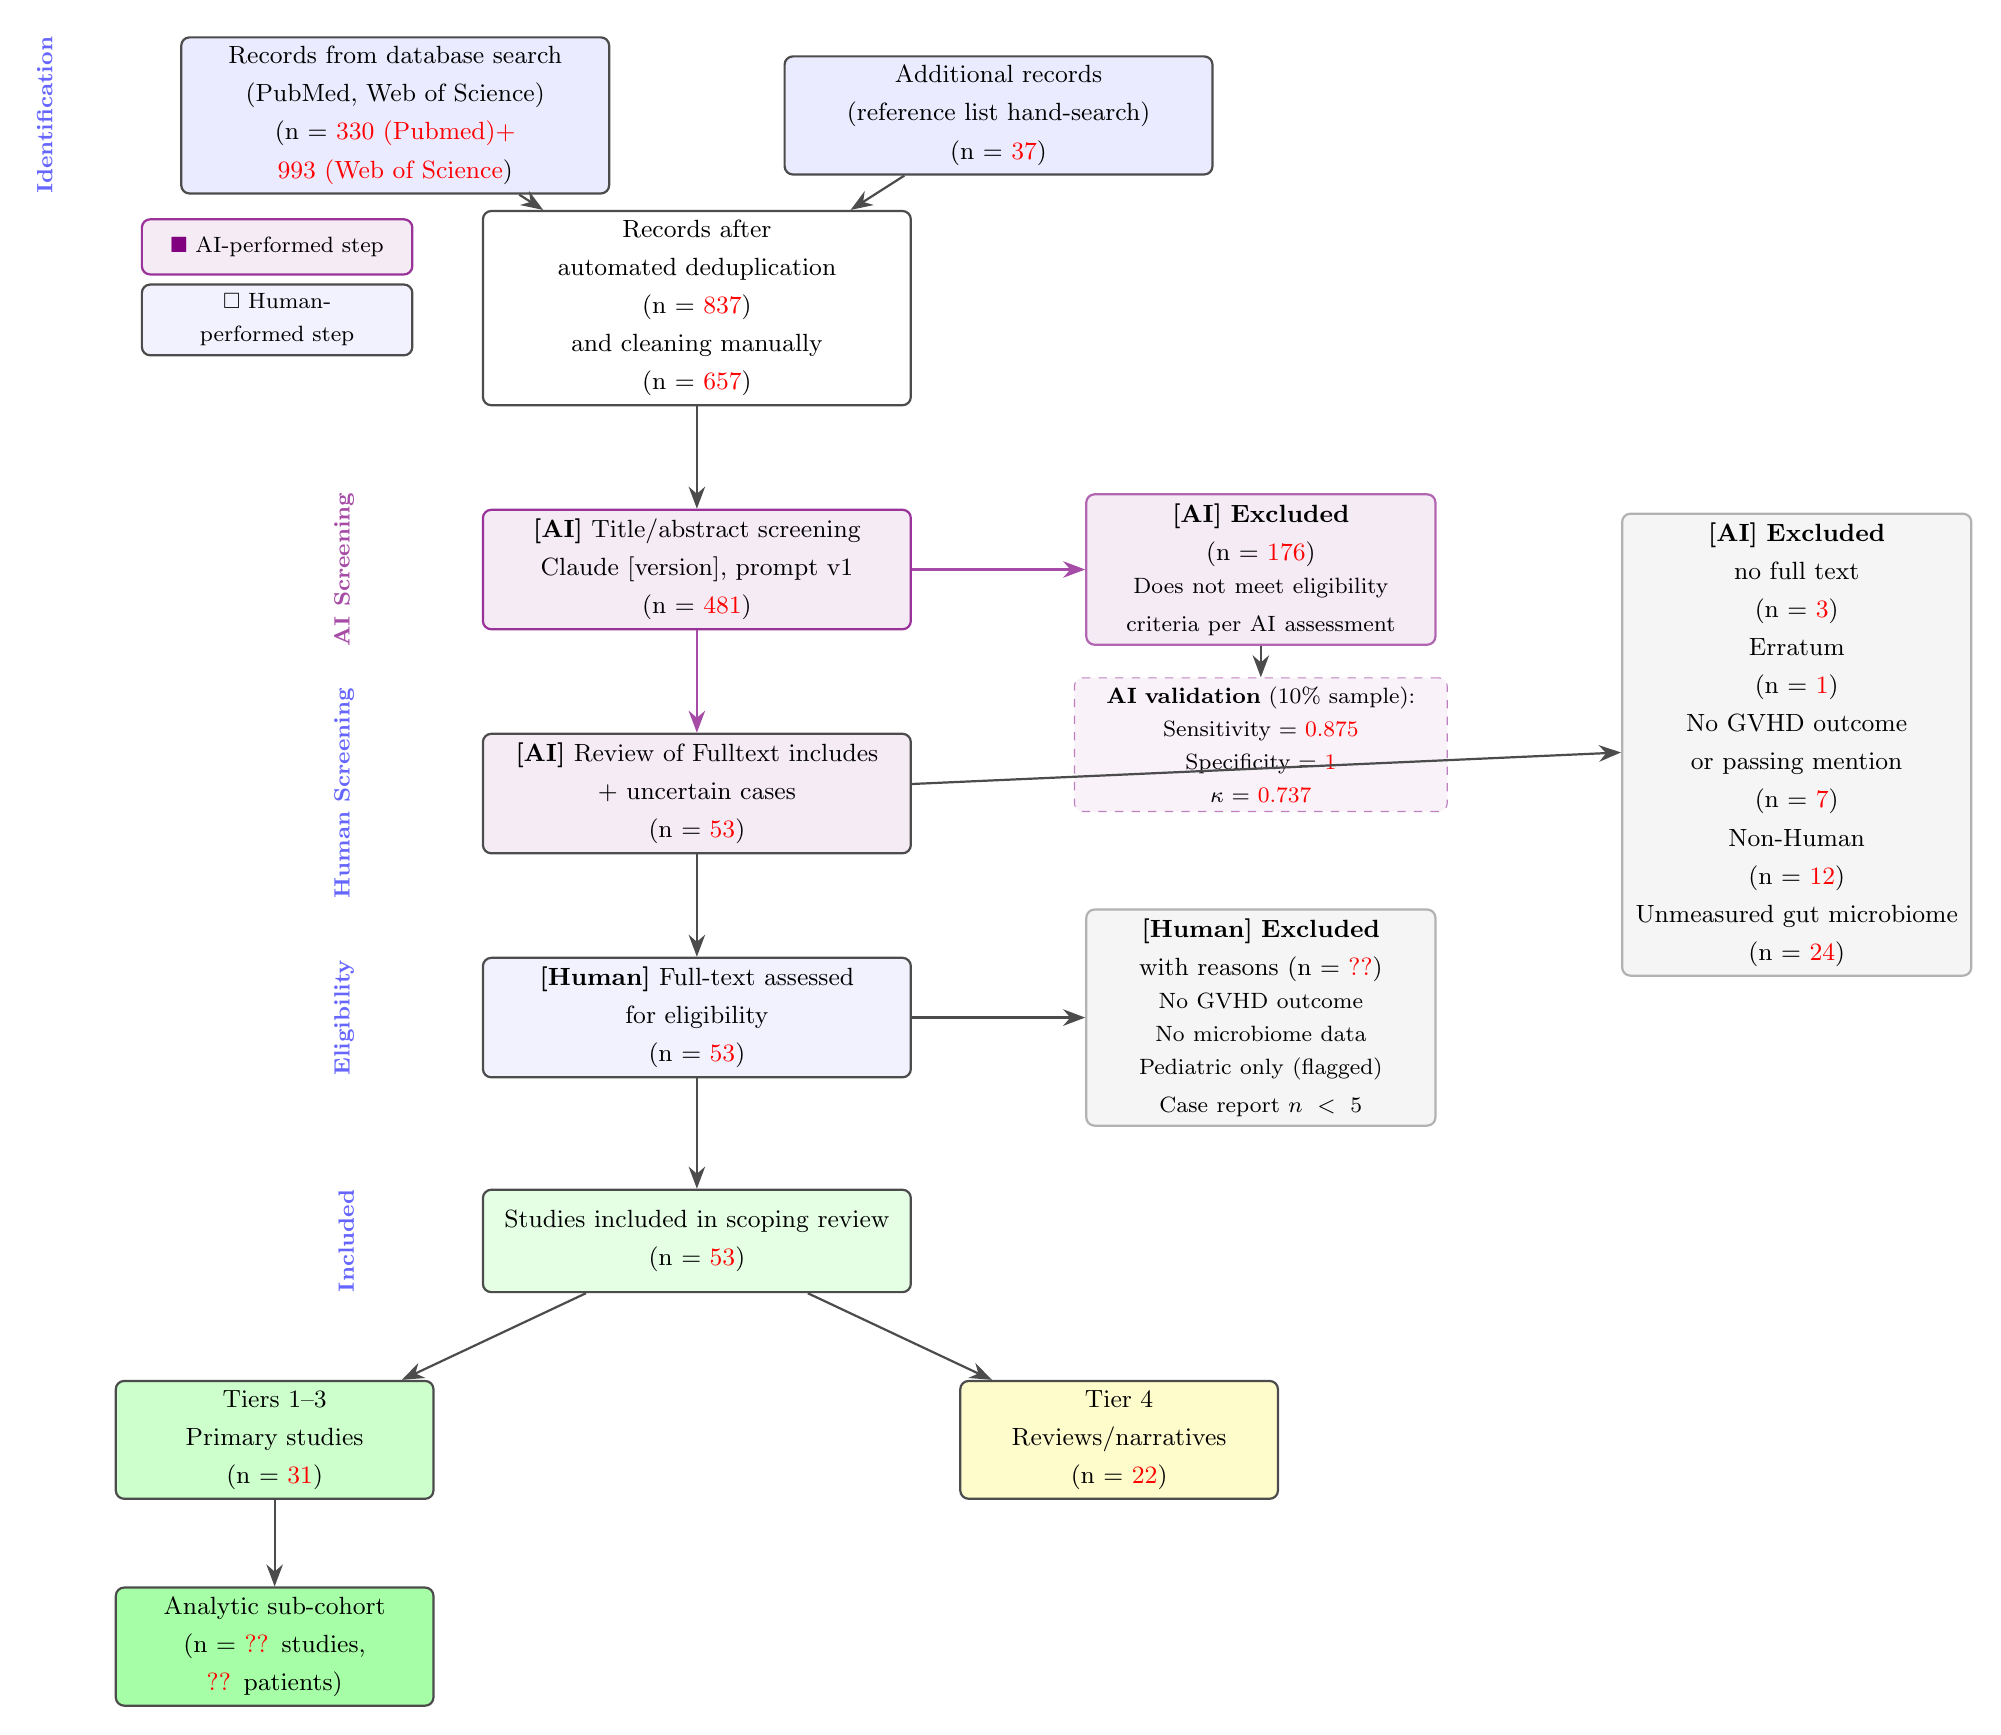
\begin{tikzpicture}[
    % Standard PRISMA boxes (human decisions)
    box/.style={rectangle, draw=black!70, thick, rounded corners=3pt,
                text width=5.2cm, minimum height=1.3cm, align=center, font=\small},
    % AI-step boxes (violet border, light fill)
    aibox/.style={rectangle, draw=violet!80, thick, rounded corners=3pt,
                  text width=5.2cm, minimum height=1.3cm, align=center,
                  font=\small, fill=violet!8},
    % Exclusion side-boxes
    excbox/.style={rectangle, draw=gray!60, thick, rounded corners=3pt,
                   text width=4.2cm, minimum height=1.1cm, align=center,
                   font=\small, fill=gray!8},
    % AI exclusion side-boxes (violet)
    aiexcbox/.style={rectangle, draw=violet!60, thick, rounded corners=3pt,
                     text width=4.2cm, minimum height=1.1cm, align=center,
                     font=\small, fill=violet!8},
    % Performance note box
    notebox/.style={rectangle, draw=violet!50, dashed, rounded corners=3pt,
                    text width=4.5cm, align=center, font=\footnotesize,
                    fill=violet!5},
    arrow/.style={-{Stealth[length=2.8mm]}, thick, black!70},
    aiarrow/.style={-{Stealth[length=2.8mm]}, thick, violet!70},
    node distance=1.3cm
]

%-------- IDENTIFICATION --------
\node[box, fill=blue!8] (id) {Records from database search\\(PubMed, Web of Science)\\(n~=~\textcolor{red}{330 (Pubmed)+ 993 (Web of Science})};
\node[box, fill=blue!8, right=2.2cm of id] (other) {Additional records\\(reference list hand-search)\\(n~=~\textcolor{red}{37})};
\node[box, below=1.2cm of $(id)!0.5!(other)$] (dedup) {Records after \\
automated deduplication \\(n~=~\textcolor{red}{837}) \\ and cleaning manually \\ (n~=~\textcolor{red}{657})};

%-------- SCREENING: AI STAGE --------
\node[aibox, below=of dedup] (aiscreen)
    {\textbf{[AI]} Title/abstract screening\\
     Claude [version], prompt v1\\
     (n~=~\textcolor{red}{481})};
\node[aiexcbox, right=2.2cm of aiscreen] (aiexcl)
    {\textbf{[AI] Excluded}\\
     (n~=~\textcolor{red}{176})\\
     {\footnotesize Does not meet eligibility\\criteria per AI assessment}};
\node[notebox, below=0.4cm of aiexcl] (aiperf)
    {\textbf{AI validation} (10\% sample):\\
     Sensitivity~=~\textcolor{red}{0.875}\\
     Specificity~=~\textcolor{red}{1}\\
     $\kappa$~=~\textcolor{red}{0.737}};

%-------- SCREENING: HUMAN VERIFICATION --------
\node[box, fill=violet!8, below=of aiscreen] (humanscreen)
    {\textbf{[AI]} Review of Fulltext includes\\
     + uncertain cases\\
     (n~=~\textcolor{red}{53})};
\node[excbox, right=2.2cm of aiperf] (humanexcl)
    {\textbf{[AI] Excluded}\\
     no full text\\
     (n~=~\textcolor{red}{3})\\
    Erratum\\
     (n~=~\textcolor{red}{1})\\
    No GVHD outcome or passing mention \\
     (n~=~\textcolor{red}{7})\\
    Non-Human\\
     (n~=~\textcolor{red}{12})\\
    Unmeasured gut microbiome\\
     (n~=~\textcolor{red}{24})};

%-------- ELIGIBILITY: FULL-TEXT --------
\node[box, fill=blue!5, below=of humanscreen] (elig)
    {\textbf{[Human]} Full-text assessed\\
     for eligibility\\
     (n~=~\textcolor{red}{53})};
\node[excbox, right=2.2cm of elig] (excl2)
    {\textbf{[Human] Excluded}\\
     with reasons (n~=~\textcolor{red}{??})\\
     {\footnotesize No GVHD outcome\\
     No microbiome data\\
     Pediatric only (flagged)\\
     Case report $n<5$}};

%-------- INCLUDED --------
\node[box, fill=green!10, below=1.4cm of elig] (incl)
    {Studies included in scoping review\\(n~=~\textcolor{red}{53})};

%-------- TIERS --------
\node[box, fill=green!20, below left=1.1cm and 0.6cm of incl, text width=3.8cm]
    (t13) {Tiers 1--3\\Primary studies\\(n~=~\textcolor{red}{31})};
\node[box, fill=yellow!20, below right=1.1cm and 0.6cm of incl, text width=3.8cm]
    (t4)  {Tier 4\\Reviews/narratives\\(n~=~\textcolor{red}{22})};

%-------- ANALYTIC SUB-COHORT --------
\node[box, fill=green!35, below=1.1cm of t13, text width=3.8cm]
    (sub) {Analytic sub-cohort\\(n~=~\textcolor{red}{??} studies,\\\textcolor{red}{??} patients)};

%-------- ARROWS: main flow --------
\draw[arrow] (id)          -- (dedup);
\draw[arrow] (other)       -- (dedup);
\draw[arrow] (dedup)       -- (aiscreen);
\draw[aiarrow] (aiscreen)  -- (humanscreen);
\draw[arrow]  (humanscreen)-- (elig);
\draw[arrow]  (elig)       -- (incl);
\draw[arrow]  (incl)       -- (t13);
\draw[arrow]  (incl)       -- (t4);
\draw[arrow]  (t13)        -- (sub);

%-------- ARROWS: exclusions --------
\draw[aiarrow] (aiscreen)    -- (aiexcl);
\draw[arrow]   (aiexcl)      -- (aiperf);
\draw[arrow]   (humanscreen) -- (humanexcl);
\draw[arrow]   (elig)        -- (excl2);

%-------- PHASE LABELS --------
\node[rotate=90, anchor=south, font=\footnotesize\bfseries, text=blue!60]
    at ($(id.west)+(-1.5,0)$)          {Identification};
\node[rotate=90, anchor=south, font=\footnotesize\bfseries, text=violet!70]
    at ($(aiscreen.west)+(-1.5,0)$)    {AI Screening};
\node[rotate=90, anchor=south, font=\footnotesize\bfseries, text=blue!60]
    at ($(humanscreen.west)+(-1.5,0)$) {Human Screening};
\node[rotate=90, anchor=south, font=\footnotesize\bfseries, text=blue!60]
    at ($(elig.west)+(-1.5,0)$)        {Eligibility};
\node[rotate=90, anchor=south, font=\footnotesize\bfseries, text=blue!60]
    at ($(incl.west)+(-1.5,0)$)        {Included};

%-------- LEGEND --------
\node[box, fill=violet!8, draw=violet!80, text width=3.2cm, minimum height=0.7cm,
      font=\footnotesize, anchor=north west]
    at ($(id.south west)+(-0.5,-0.3)$) (leg_ai)
    {\textcolor{violet}{$\blacksquare$} AI-performed step};
\node[box, fill=blue!5, draw=black!70, text width=3.2cm, minimum height=0.7cm,
      font=\footnotesize, anchor=north west]
    at ($(leg_ai.south west)+(0,-0.1)$)
    {$\square$ Human-performed step};

\end{tikzpicture}
}% end resizebox
\caption{\textbf{PRISMA-trAIce modified flow diagram.}
Study identification, screening, and inclusion process following PRISMA-ScR guidelines with the PRISMA-trAIce extension for transparent AI reporting.
Violet nodes represent steps performed by AI (Claude); blue nodes represent human-performed steps.
The screening stage is split per PRISMA-trAIce requirements: AI exclusions and human exclusions are tracked separately.
The AI validation box reports screening performance on a random 10\% human gold-standard subsample.
Numbers to be filled after search and screening are complete.
Studies are categorized into Tiers 1--4; the analytic sub-cohort additionally requires time-to-GVHD outcomes and publicly available 16S data.}
\label{fig:prisma}
\end{figure}


\todoitem{Report total records identified, deduplicated, screened, included.}
\todoitem{Breakdown by tier.}
\todoitem{Common exclusion reasons.}

\end{document}

